\documentclass[12pt]{ociamthesis}  % default square logo 
%\documentclass[12pt,beltcrest]{ociamthesis} % use old belt crest logo
%\documentclass[12pt,shieldcrest]{ociamthesis} % use older shield crest logo

%load any additional packages
\usepackage{amssymb}
\usepackage{amsmath}
\usepackage{bbm}
\usepackage{graphicx}
\graphicspath{ {./images/} }
%input macros (i.e. write your own macros file called mymacros.tex 
%and uncomment the next line)
%\include{mymacros}

\title{Modelling and analysis of social network data from rank preferences     %your thesis title,
	}   %note \\[1ex] is a line break in the title

\author{Pierre OSSELIN}             %your name
\college{St Peter's College}  %your college

%\renewcommand{\submittedtext}{change the default text here if needed}
\degree{MSc in Mathematical Sciences}     %the degree
\degreedate{Trinity 2018}         %the degree date

%end the preamble and start the document
\begin{document}
	
	
	\maketitle                  % create a title page from the preamble info
	\tableofcontents
	
	
	%now include the files of latex for each of the chapters etc
	\chapter{Introduction}
	This paper aims at performing inference on social network through partial ranking of the individuals
	
	We use the Plackett-Luce model: 
	\begin{equation}
		p(\rho_{i} | (\lambda)) = \prod_{k = 1}^{K}\frac{\lambda_{i\rho_{k}}}{\sum_{j \neq i}\lambda_{i,j} - \sum_{l = 1}^{k - 1}\lambda_{i,\rho_{l}}}
	\end{equation}
	Where $K$ is the number of ranked individuals. This model is equivalent to successively choose our favorite individual by pondering our strength of affiliation with each person, and take randomly the best remaining by taking into account the proportion of this strength among the other, which is a conceivable model.
	
	The first thing to do is to prove that Plackett-Luce is well defined as a probability distribution. It is easy to prove it by induction over $K \leq n$. We denote $\Omega_{K,n} := \{ \rho : \{1,...,K\} \rightarrow I_{K} \ bijective, I_{K} \in [n]^{(K)}  \}$. For $K = 1 :$
	
	\begin{equation}
	\sum_{\rho \in \Omega_{1,n} }p(\rho | (\lambda)) = \sum_{k \neq i}\frac{\lambda_{i,k}}{\sum_{j \neq i}\lambda_{i,j}} = 1
	\end{equation}
	
	If the result is true for $K - 1 < n$ then, with $\forall j \neq i, \Omega_{K,n,j} = \{ \rho : \{1,...,K\} \rightarrow I_{K} \ bijective, I_{K} \in [n]^{(K)}, \rho(1) = j\}$ and $\hat{(\lambda)}_{j}$ the matrix without column $j$:
	\begin{equation}
	\sum_{\rho \in \Omega_{K,n} }p(\rho | (\lambda)) = \sum_{j = 1}^{n} \sum_{\rho \in \Omega_{K,n,j}}p(\rho | (\lambda))
	\end{equation}
	
	\begin{equation}
	= \sum_{j = 1}^{n} \frac{\lambda_{i,j}}{\sum_{l \neq i}\lambda_{i,l}} \underbrace{\sum_{\rho \in \Omega_{K-1,n-1}}p(\rho | \hat{(\lambda)}_{j})}_\text{= 1 by induction} = 1
	\end{equation}
	
	
	\chapter{Community representation}
	\section{Mathematic Formulation}
	Here we suppose that the strength between individuals are characterized by their similitude to certain communities.
	
	We introduce $p$ the number of communities and $(w_{i,k})_{1 \leq i \leq n,1 \leq k \leq p }$ the strength of affiliation of the individual $i$ to the community $p$.
	\begin{equation}
	\lambda_{i,j} = \sum_{k = 1}^{p} w_{i,k} w_{j,k}
	\end{equation}
	
	This formulation is equivalent to the rank matrix approximation often encountered in the literature where we assume that:
	
	\begin{equation}
	(\lambda) = WW^{T}
	\end{equation} where $W$ is the matrix of the $(w_{i,k})$
	
	We suppose here that the strength of the relations are only determined by the proximity with a certain community hence that the relations are reciprocal.
	From the reordering inequality, we can observe that $\lambda_{i,j}$ is maximized when both $i$ and $j$ have the same community ranking preferences.
	We can interpret the formula $\lambda_{i,j} = \sum_{k = 1}^{p} w_{i,k} w_{j,k}$ also as a scalar product in the p-dimensional space of communities. In this space, each individual is a point represented by a vector $w_{i} \in (\mathbb{R}^{+})^{p} $ the strength of affiliation is also computed by $\lambda_{i,j} = ||w_{i}||.||w_{j}||.cos(\theta)$ we can interpret the norm of the vector as the individual global influence or sociability, and the $\theta$ as the divergence in personality. Hence a given individual will appreciate another individual with great sociability but different personality or views as much as a low sociability individual with the same mindset.
	In this interpretation, the prior function attributed to the $w_{i,k}$ is equivalent to putting a topography on the space, allowing points to lie more likely in a certain area.
	This is illustrated in the Figure \ref{label-image7}
	
	The main issue regarding this geometric approach is that having a bigger affiliation means that the community points have a greater scalar product, but doesn't mean those points are nearer. If we wanted to use a clustering approach to this problem, we should build a space in which the mapping to this space make it equivalent having great scalar product in the input space and being near in the output space.
	\begin{figure}
		\centering
		\begin{minipage}{0.45\textwidth}
			\centering
			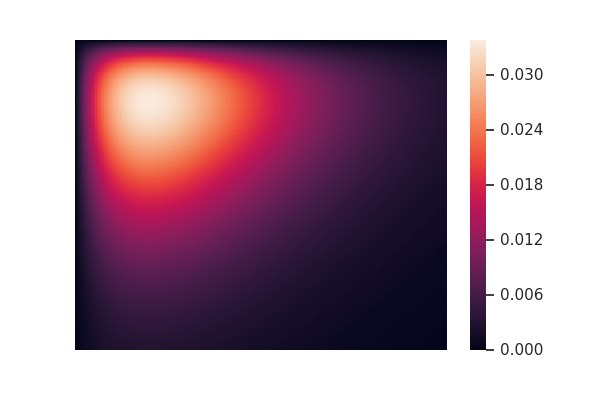
\includegraphics[width=0.9\textwidth]{heatMap} % first figure itself
			\caption{Topography of the community space for the same gamma distribution}
			\label{label-image7}
		\end{minipage}\hfill
		\begin{minipage}{0.45\textwidth}
			\centering
			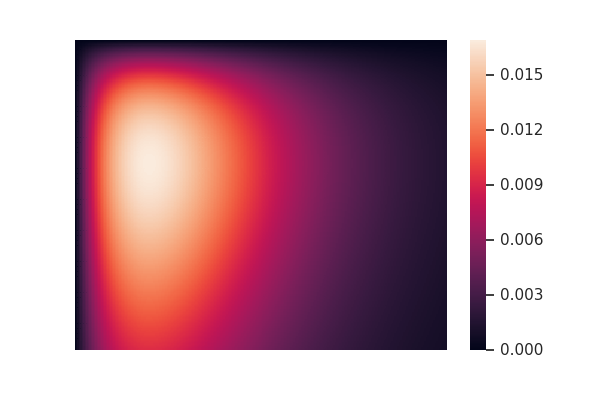
\includegraphics[width=0.9\textwidth]{heatMapCorrection} % second figure itself
			\caption{Topography of the community space for different gamma distribution}
			\label{label-image8}
		\end{minipage}
	\end{figure}


	\section{Computation of the posterior}
	Let's define the log-posterior of the community representation. Which is the sum of the log priors of the parameters and the log-likelihood. 
	\begin{equation}
	l((w);D) = \sum_{i = 1}^{n} \sum_{k = 1}^{p} (\alpha - 1)ln(w_{i,k}) - \beta w_{i,k} + \sum_{i = 1}^{n} \sum_{j = 1}^{K} ln(\lambda_{i,\rho_{j}}) - ln(\sum_{j \neq i} \lambda_{i,j} - \sum_{l = 1}^{j-1} \lambda_{i,\rho_{l}})
	\end{equation}
	
	To make the optimization easier, we can compute the gradient of the posterior according to the parameter $w_{r,s}$
	
	With 
	\begin{equation}
	\frac{\partial \lambda_{i,j}}{\partial w_{r,s}} = 1_{i = r} w_{j,s} + 1_{j = r} w_{i,s}
	\end{equation}
	We have :
	
	\begin{multline}
	\frac{\partial l((w);D)}{\partial w_{r,s}} = \frac{a-1}{w_{r,s}} - b + \sum_{j = 1}^{K} \frac{1}{\lambda_{r,\rho^{(r)}_{j}}} w_{\rho^{(r)}_{j},s} + \sum_{i = 1; i \neq r}^{n} \sum_{j = 1}^{K} \frac{1}{\lambda_{i,r}} w_{i,s} 1_{\rho^{(r)}_{j} = r} - \\ \sum_{j = 1}^{K} \frac{1}{\sum_{j \neq r} \lambda_{r,j} - \sum_{l = 1}^{j - 1} \lambda_{r,\rho^{(r)}_{l}}} \sum_{j \neq r} w_{j,s} - \sum_{i = 1; i \neq r}^{n} \sum_{j = 1}^{K} \frac{1}{\sum_{j \neq i} \lambda_{i,j} - \sum_{l = 1}^{j - 1} \lambda_{i,\rho^{(i)}_{l}}} w_{i,s} + \\ \sum_{j = 1}^{K} \frac{1}{\sum_{j \neq r} \lambda_{r,j} - \sum_{l = 1}^{j - 1} \lambda_{r,\rho^{(r)}_{l}}} \sum_{l = 1}^{j-1} w_{\rho^{(r)}_{l},s} + \sum_{i = 1; i \neq r}^{n} \sum_{j = 1}^{K} \frac{1}{\sum_{j \neq i} \lambda_{i,j} - \sum_{l = 1}^{j - 1} \lambda_{i,\rho^{(i)}_{l}}} \sum_{l = 1}^{j - 1} 1_{\rho^{(i)}_{l} = r} w_{i,s}	
	\end{multline}

	\begin{figure}
		\centering
		%		\textbf{Your title}\par\medskip
		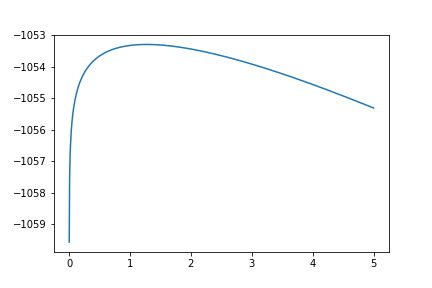
\includegraphics[width=\textwidth,height=\textheight,keepaspectratio]{CoordinateWiseFunction}
		\caption{Posterior according to one coordinate}
	\end{figure}
	
	\section{Simulations on simulated Data}
	\subsection{Fixed parameters for the prior}
	We derived two optimization algorithm to find the MAP, one based on coordinate-wise optimization, given that for the a and b considered, the log-posterior seems coordinate-wise concave, hence assuring a more stable convergence. The other algorithm is based on the L-BFGS-B algorithm, popular in machine learning optimization.
	
	For this simulation we took $a = 2$, $b = 1$ $n = 15$, $p = 3$, $k = 3$ , drew a sample from $w$, computed $\lambda$ and $\rho$. Then we maximized the posterior according to the two methods described above, in order to estimate the community strengths and then the individual mutual strength. 
%		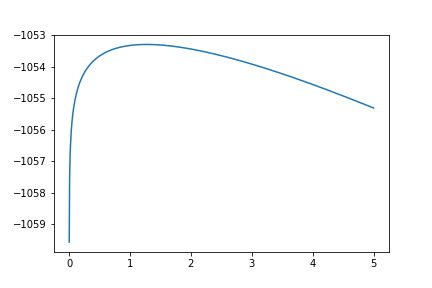
\includegraphics[width=\textwidth,height=\textheight,keepaspectratio]{CoordinateWiseFunction}

%	\begin{figure}
%		\centering
%%		\textbf{Your title}\par\medskip
%		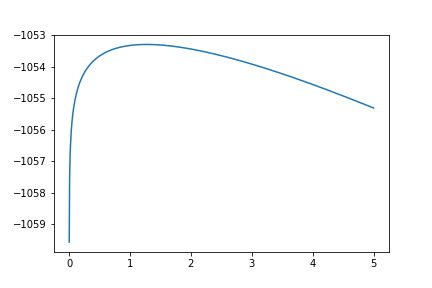
\includegraphics[width=\textwidth,height=\textheight,keepaspectratio]{CoordinateWiseFunction}
%			\caption{Posterior according to one coordinate}
%	\end{figure}

	\begin{figure}
		\centering
		%		\textbf{Your title}\par\medskip
		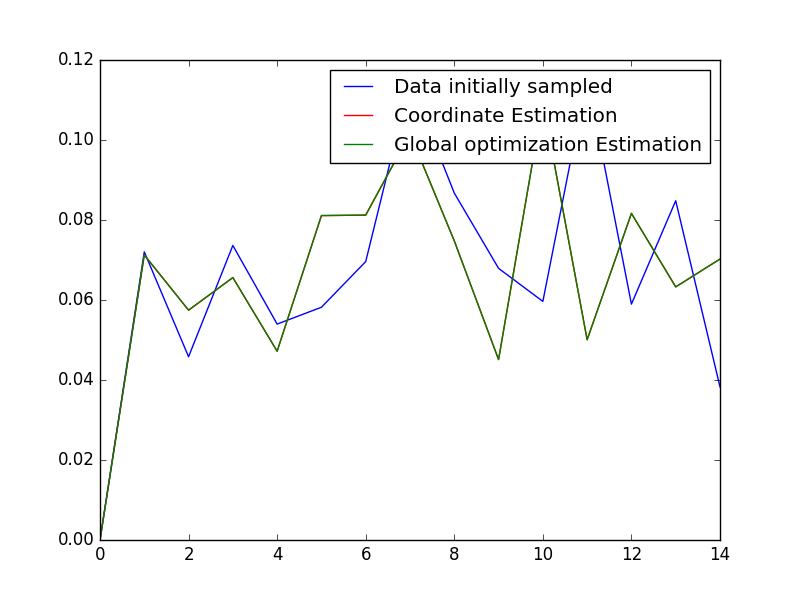
\includegraphics[width=\textwidth,height=\textheight,keepaspectratio]{LambdaEstimation}
		\caption{Comparison between the sampled and estimated Social affiliation of the first individual}
		\label{label-image1}
	\end{figure}
	
	In figure \ref{label-image1} we can see that the coordinate and global optimization have converged to the same result. We obtain an absolute error of 0.02. Which is equivalent to 0.3 reported to the number of individual, and a ranking gap (mean absolute ranking error) of 2.13 for this individual.
	
	It is interesting to compare the ranking gap to the expected ranking gap from a random permutation. We can manually compute with a tedious calculation that
	\begin{center}
		\resizebox{8cm}{!}{$ \frac{1}{n} \mathbb{E}_{\mathbb{\sigma}_{n}}[ \sum_{k = 1}^{n} |\sigma(k) - k| ] = \frac{n^{2} - 1}{3n} $}
	\end{center}
	
	For n = 18 we have a random expectation of the ranking gap of 6. Hence the model tends to preserve the "global" social network for each individual.
	
	\begin{figure}
		\centering
		%		\textbf{Your title}\par\medskip
		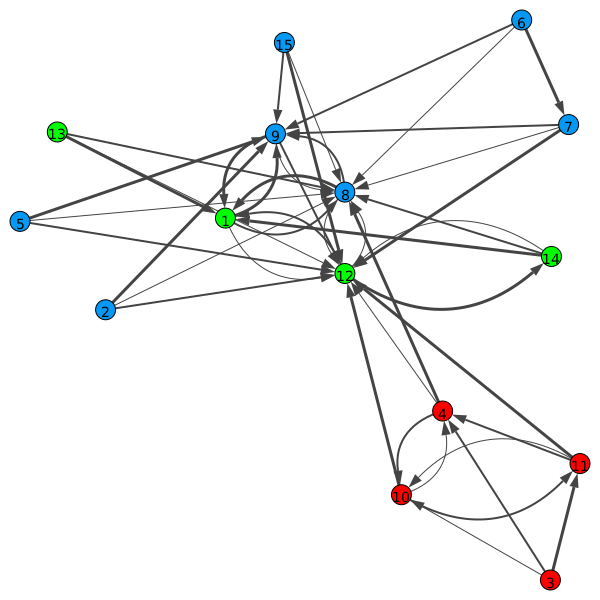
\includegraphics[width=\textwidth,height=\textheight,keepaspectratio,scale=0.5]{OriginalPlot}
		\caption{Original Community description}
		\label{label-image2}
	\end{figure}

	\begin{figure}
		\centering
		%		\textbf{Your title}\par\medskip
		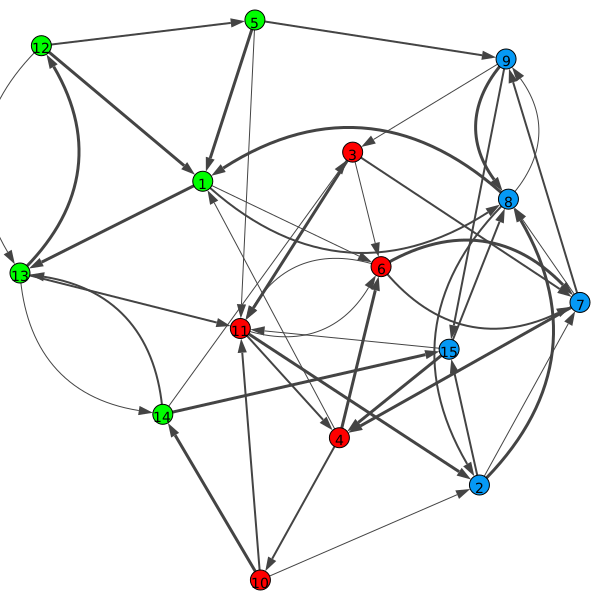
\includegraphics[width=\textwidth,height=\textheight,keepaspectratio]{OptimizationPlot}
		\caption{Inferred community}
		\label{label-image3}
	\end{figure}
	
	We can see that the inferred communities are quite similar to the original one. The original red and green communities are preserved except for the individual 6 and 5 that has passed from the blue community to the red and green respectively. Here we have assigned an individual to his preferred community, the width of an edge represents the importance the son represents for the father.
	\subsection{Model with degree-correction}
	
	In this subsection, we try to capture the different popularity that a community can have over the other communities. In the previous model, the regularization terms $w_{i,j}$ in the posterior had the same weights, irrespective of the community concerned (Having a too big $w_{i,j}$ was equally improbable regardless of the community). In a model with degree-correction, i.e in which $w_{i,k} \sim  \Gamma(\alpha, \beta_{k})$, we do not prevent the possibility of a popular community in the regularization, which occurs by the emergence of popular individuals.
	\begin{figure}
		\centering
		%		\textbf{Your title}\par\medskip
		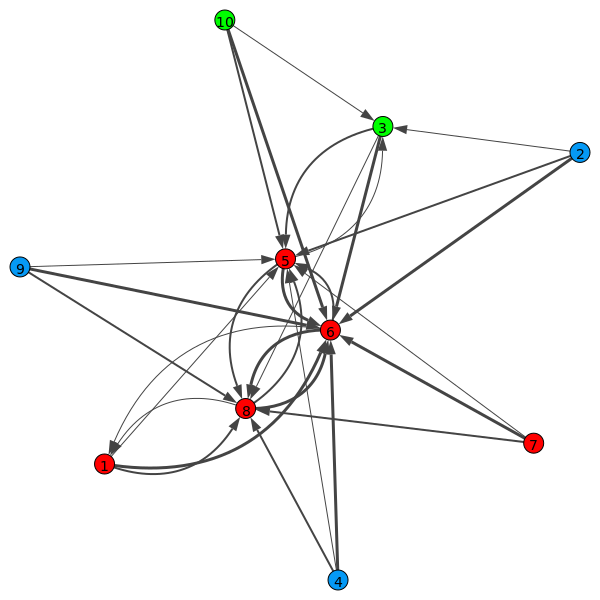
\includegraphics[width=\textwidth,height=\textheight,keepaspectratio]{OriginalPlotDegreeCorrection}
		\caption{Original Community description for the degree Correction Model}
		\label{label-image5}
	\end{figure}
	
	\begin{figure}
		\centering
		%		\textbf{Your title}\par\medskip
		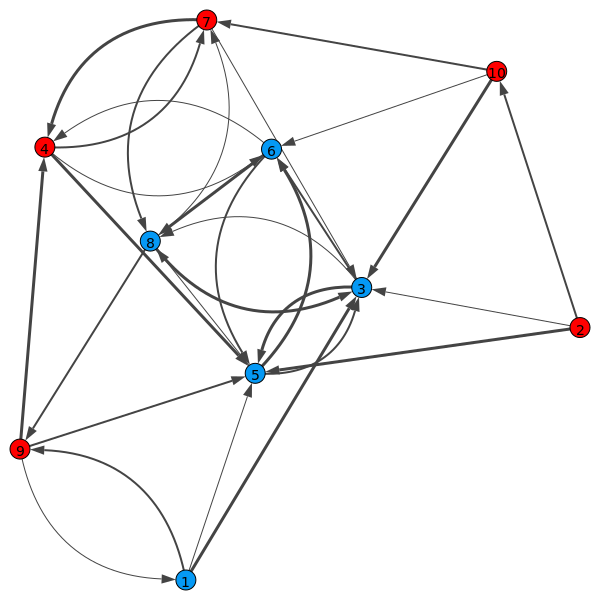
\includegraphics[width=\textwidth,height=\textheight,keepaspectratio]{OptimizationPlotDegreeCorrection}
		\caption{Inferred community for the degree correction Model}
		\label{label-image6}
	\end{figure}
	
	
	We can see in this example that the green community has been absorbed in an other community by the inference, and that 7 has been replaced by 3 in the other community.
	
	\subsection{Performance Comparison}
	
	To evaluate the performance of the models, we make prediction on the preferences for individuals who have not indicated their preferences, provide further preferences from individuals who did, or extract from the lists interpretable information about the structure of the underlying friendship network, e.g. in terms of latent communities. For this we will use different metrics. The ranking gap between latent appreciation, the absolute error in the strengths and the missed community. To do that, we will sample the strengths between individuals $\lambda_{i,j}$ and then sample full rankings from it. From this ranking we then hide a certain part of it, we feed the remaining parts to our model and then compute the error in terms of metrics previously defined to evaluate the performance.
	
	\chapter{Model with Covariates}
	
	The purpose of ERGMs, in a nutshell, is to describe parsimoniously the local selection forces
	that shape the global structure of a network. To this end, a network dataset, like those
	depicted in Figure 1, may be considered like the response in a regression model, where the
	predictors are things like “propensity for individuals of the same sex to form partnerships” or
	“propensity for individuals to form triangles of partnerships”. In Figure 1(b), for example, it
	is evident that the individual nodes appear to cluster in groups of the same numerical labels
	(which turn out to be students’ grades, 7 through 12); thus, an ERGM can help us quantify
	the strength of this intra-group effect. The information gleaned from use of an ERGM may
	then be used to understand a particular phenomenon or to simulate new random realizations
	of networks that retain the essential properties of the original. Handcock, Hunter, Butts,
	Goodreau, and Morris (2008) say more about the purpose of modeling with ERGMs; yet in
	this article, we focus primarily on technical details.
	
	\section{Notation}
	Let $N$ be the set of nodes in the network of interest, indexed $\{ 1,...,n\}$ The relationships in
	the network may be directed (e.g., friendship nominations, messages) or undirected (e.g., sexual
	partnerships, conversations). In the former case, we define the set of dyads (here used to refer
	to potential relationships) $\mathbb{Y}$ to be a subset of $N \times N$, the set of ordered pairs of nodes; in the
	latter case, it is a subset of $\{ \{i, j\} : (i, j) \in N \times N\}$, the unordered pairs of nodes. (We will also
	use u($\mathbb{Y}$) to refer to an “unordered” version of $\mathbb{Y}$, i.e., u($\mathbb{Y}$) $\equiv$ $\{\{i, j\} : (i, j) \in Y \}$.) Usually, $\mathbb{Y}$ is
	further constrained in that in most social networks studied, a node cannot have a relationship of
	interest with itself, excluding pairs of the form $(i, i)$.
	For binary networks, in which the relationship of interest must be either present or absent,
	we use $\mathcal{Y}$ $\in$ $2^{\mathbb{Y}}$
	, the set of subsets of $\mathbb{Y}$, to refer to the set of possible networks of interest, which may be further constrained (that is, $\mathbb{Y}$ may be a proper subset of $2^{\mathbb{Y}}$). We will use $\textbf{Y}$ to refer to
	network random variables and $y$ $\in$ $\mathcal{Y}$ to refer to their realizations, and $y_{i,j}$ be an 0 - 1 indicator of
	whether a relationship of interest is present between i and j in a binary network context.
	
	
	\section{ERGM model}
	In the ERGM model (exponential-family random graph models), the distribution of $\textbf{Y}$ can be parameterized in the form:
	
	\begin{equation}
	P_{\theta}(Y = y) = \frac{exp((\eta(\theta)) ^{T}*z(x))}{\chi(\theta)}, y \in \mathcal{Y}
	\end{equation}
	
	where $\theta$ is a q-vector of model parameters, which are mapped to a p-vector of natural parameters
	by $\eta(.)$, and $g(.)$ is a p-vector of sufficient statistics, which capture network features of interest. These sufficient statistics typically embody the
	features of the network of interest that are believed to be significant to the social
	process which had produced it, such as degree distribution (e.g., propensity
	towards monogamy in sexual partnership networks), homophily (i.e., “birds of
	a feather flock together”), and triad-closure bias (i.e., “a friend of a friend is a
	friend”) . (Morris, Handcock and Hunter, 2008)
	
	\section{The $p1$ Model}
	
	The $p_{1}$ model is the first to propose log-linear models for social
	networks. Suppose that we take $\mathcal{Y}$ to be the set of all directed graphs, with independent dyads [i.e., the pairs ($Y_{i,j}$ , $Y_{j,i}$ ) are independent for different choices of $\{i, j\}$] and the following model for tie probabilities:
	
	\begin{multline}
	P(Y_{i,j} = y_{1}, Y_{j,i} = y_{2}) = exp \{ y_{1}(\mu + \alpha_{i} + \beta_{j}) + y_{2}(\mu + \alpha_{j} + \beta_{i}) + y_{1}y_{2} \rho\} \backslash k_{ij} \\  y_{1}, y_{2} = 0,1 ; i,j = 1,...,n; i \neq j 
	\end{multline}
	
	In this model, we can interpret $\mu$ as a density parameter, constituting an overall mean, $\alpha_{i}$ as a productivity parameter, characterizing i as a sender, $\beta_{j}$ as an attractiveness parameter, characterizing j as a receiver, and $\rho$ as a parameter indicating the force of reciprocation.
	
	\section{The $p2$ Model}
	
	While ERGMs are useful for modeling global network characteristics, models based on conditional independence (given latent variables) are useful for multiple reasons. First, ERGMs are not well understood and sometimes possess undesirable properties, e.g., model degeneracy. Second, the likelihood function of ERGMs is intractable, complicating statistical computing. Third, there may be unobserved heterogeneity or unobserved structure.
	Models based on independence conditional on latent variables: random effects models and mixed effects models and extensions; stochastic block models and extensions, including mixed membership models; and latent space models and extensions.
	
	The aim of the $p_{2}$ model is to relate binary network data to covariates while taking into account the specific network structure. This requires a kind of bivariate logistic regression model capable of handling the dependence of network data.
	The $p_{2}$ model is based on the same formula. The density and reciprocity parameters, however, are allowed to vary over dyads, and are therefore denoted $\mu_{ij} $ and $\rho_{ij}$. Moreover, parameters $\alpha_{i}$ , $\beta_{j}$ , $\mu_{ij}$ , and $\rho_{ij}$ are further modelled using covariates.
	We first consider the node-specific parameters $\alpha_{i}$ and $\beta_{j}$. Covariates and random effects are included in a linear regression model for the productivity and attractiveness parameters.
	
	\begin{equation}
	\begin{cases}
	\alpha = X_{1} \gamma_{1} + A \\
	\beta = X_{2} \gamma_{2} + B
	\end{cases}
	\end{equation}

	This formulation expresses the plausible idea that attractiveness (or popularity) and productivity (or sociability) depend on actor attributes (denoted by $X_{1}$ and $X_{2}$ , respectively, where the same or different attributes may be used for attractiveness and productivity) with corresponding weights $\gamma_{1}$ and $\gamma_{1}$ . Naturally, the attributes do not explain all variation in attractiveness and productivity parameters, as is represented by the residual terms A and B, n $\times$ 1 vectors with components $A_{i}$ and $B_{i}$ . The residuals are modeled as normally distributed random variables with expectation 0 and variances $\sigma_{A}^{2}$ and $\sigma_{B}^{2}$ , respectively. Parameters $\sigma_{A}^{2}$ and $\sigma_{B}^{2}$ can be interpreted as unexplained variance, that is, the variance of the $\alpha$’s and $\beta$’s that is left after taking into account the effect of the covariates $X_{1}$ and $X_{2}$ . The productivity and attractiveness parameters of the same node
	are correlated:$\forall i,  cov(A_{i} , B_{i} ) = \sigma_{AB}$. Independence is assumed for parameters of different actors by setting $cov(A_{i} , A_{j} )=cov(B_{i} , B_{j} )=cov(A_{i} , B_{j} ) = 0$ for
	$i \neq j$ (cf. Wong, 1987).
	If no external information on actors is available, the terms $X_{1} \gamma_{1}$ and $X_{2} \gamma_{2}$ vanish and $\sigma_{A}^{2}$ and $\sigma_{B}^{2}$ denote the variances of the $\alpha$ and $\beta$ parameters, respectively. Then a pure random effects model results with, apart from the density and reciprocity parameters, only two variance parameters and one covariance parameter. Thus, the $p_{2}$ model without covariates is a more parsimonious model than the $p_{1}$ model with well-interpretable parameters. Obviously, the fit of $p_{1}$
	will be better than the fit of $p_{2}$ without covariates.
	
	
	\section{The SRM Model}
	
	ERGM models models work very poorly, the learned parameters do not generate data that resembles the input and tend toward wholly connected or completely empty graphs. Similarly, Since a binary random graph model does not accommodate rank data, analysis of these data with such a model typically begins by reducing all positive ranked relations to “ones,” and all negative ranked relations to “zeros,” leaving unranked relations as zeros as well. Such a data analysis essentially throws away some of the information in the data. Furthermore, the support of most binary random graph models consists of all possible graphs on the node set. In contrast, the data collection scheme used by Sampson (1969) was censored, as no graph with more than three outgoing edges per node could have been observed.
	
	We take the same formulation as for the community representation. Latent variable $\textbf{Y}$ representing the strength of affiliation between individuals. And $\textbf{S}$ the sociomatrix given in data. $\textbf{S}$ =
	$\{ s_{i,j} : i \neq j\}$, coded so that si,j = 0 if j is not nominated by i, si,j = 1 if j is i’s least favored
	nomination, and so on. Under this coding, $s_{i,j}$ > $s_{i,k}$ if $i$ scores $j$ “more highly” than $k$, or if $i$
	nominates $j$ but not $k$. Letting $a_{i} = \{1, ..., n\} \backslash \{i\}$ be the set of individuals whom person $i$ may potentially nominate, each observed outdegree $d_{i} = \sum_{j \in a_{i}} 1(s_{i,j} > 0)$ satisfies $d_{i} \leq m$.
	
	We then write
	
	$s_{i,j} = [(m-rank_{i}(y_{i,j} + 1) \wedge 0)] \times 1(y_{i,j} > 0 )$
	
	and its inverse:
	
	$s_{i,j} > 0 \Rightarrow y_{i,j} > 0$
	
	$s_{i,j} > s_{i,k} \Rightarrow y_{i,j} > y_{i,k}$
	
	$s_{i,j} = 0$ and $d_{i} < m \Rightarrow y_{i,j} \leq 0$
	
	Given a statistical model $\{p(Y|\theta) : \theta \in \Theta \}$ for the underlying social relations Y, inference for
	the parameter θ can be based on a likelihood derived from the observed scores S. The
	likelihood is, as usual, the probability of the observed data S as a function of the parameter
	θ. To obtain this probability, let F(S) denote the set of Y-values that are consistent with S in
	terms of associations (2)–(4) above. Since the entries of S are the observed scores if and
	only if Y ∈ F(S), the likelihood is given by
	
	$L_{F}(\theta : \textbf{S}) = Pr(Y \in F(S) | \theta) = \int_{F(S)} p(Y|\theta) d\mu(Y)$ where μ is a measure that dominates the probability densities $\{p(Y|\theta) : \theta \in \Theta \}$.
	
	
	Given current values of $(\theta, Y)$, one step of the Gibbs sampler for the FRN likelihood proceeds by updating the values as follows:
	
	1) Simulate $\theta \sim p(Y|\theta)$
	2) For each $i \neq j$, simulate $y_{i,j} \sim p(y_{i,j}|\theta, Y_{-(i,j)}, Y \in F(S))$ as follows:
	
	a) if $s_{i,j} > 0$, simulate
	
	$y_{i,j} \sim p(y_{i,j}| Y_{-(i,j)},\theta) \times 1(max \{ y_{i,k} : s_{i,k} < s_{i,j} \} \leq y_{i,j} \leq min \{ y_{i,k} : s_{i,k} > s_{i,j} \} ); $
	
	b)  if $s_{i,j} = 0$, and $d_{i} < m$ simulate $y_{i,j} \sim p(y_{i,j}| Y_{-(i,j)}, \theta) \times 1(y_{i,j} \leq 0)$;
	
	c) if $s_{i,j} = 0$, and $d_{i} = m$ simulate $y_{i,j} \sim p(y_{i,j}| Y_{-(i,j)}, \theta) \times 1(y_{i,j} \leq min \{ y_{i,k} : s_{i,k} > 0 \})$;
	
	In the above steps, $"y \sim f(y)"$ means $"$ simulate $y$ from a distribution with density proportional
	to $f(y)$.$ " $ For each ordered pair (i, j), step 2 of this algorithm will generate a value of $y_{i,j}$ from
	its full conditional distribution, constrained so that conditions (2)–(4) that define the FRN likelihood are met.
	
	To deal with the previous remarks, we apply a model in the case where $\theta$  represents the parameters in the following standard regression model for relational data:
	
	$y_{i,j} = $ \boldmath $\beta^{T} {x_{i,j}}$ \unboldmath + $a_{i} + b_{j} + \epsilon_{i,j}$
	
	\(
	\begin{pmatrix}
	a_{i} \\
	b_{i}
	\end{pmatrix}
	\), i = 1,...,n $\sim $ i.i.d normal(0,$\Sigma_{ab}$)
	
	\(
	\begin{pmatrix}
	\epsilon_{i,j} \\
	\epsilon_{j,i}
	\end{pmatrix}
	\), i = 1,...,n $\sim $ i.i.d normal(0,$\sigma^{2}$ $\begin{pmatrix} 1 & \rho \\ \rho & 1 \end{pmatrix}$)
	
	The additive row effect $a_{i}$ is often interpreted as a measure of person $i$’s "sociability" whereas the additive column effect $b_{i}$ is taken as a measure of $i$’s "popularity.". The parameter $\rho$ represents potential correlation between $y_{i,j} $ and $y_{j,i}$. In a mixed-effects version
	of this model, the possibility that a person’s sociability $a_{i}$ is correlated with their popularity $b_{i}$ can be represented with a covariance matrix $\Sigma_{ab}$. The covariance among the elements of $Y = {y_{i,j} : i \neq j}$ induced by $\Sigma_{ab}$ and is called the SRM (Warner et al. ,1979).
	
	\section{Plackett-Luce Model with Covariates}
	
	To adapt a model with covariates to the Bradley-Terry likelihood wi will model the strength matrix as follow:
	
	$log(y_{i,j}) = $ \boldmath $\beta^{T} {x_{i,j}}$ \unboldmath + $a_{i} + b_{j} + \epsilon_{i,j}$
	
	\(
	\begin{pmatrix}
	\epsilon_{i,j} \\
	\epsilon_{j,i}
	\end{pmatrix}
	\), i = 1,...,n $\sim $ i.i.d normal(0,$\sigma^{2}$ $\begin{pmatrix} 1 & \rho \\ \rho & 1 \end{pmatrix}$)
	
	
	We will treat \boldmath $\beta$ \unboldmath, \boldmath $a$ \unboldmath \boldmath $b$ \unboldmath and $\Sigma_{\epsilon}$ as parameters.
	
	To perform bayesian inference, we need to compute an integral over a high dimensional, and intractable set of $(\lambda)$.
	
	$L(\theta | (\rho)) \propto p(\theta)p((\rho) | \theta) = p(\theta)\int_{(\lambda)}p((\lambda) | \theta)p((\rho) | (\lambda)  $
	
	
	Given the observed ranks $(\rho)$ and a prior distribution $p(\theta)$ over the parameter space, the joint posterior distribution with density $p(\theta, (\lambda)|(\rho)$ can be approximated by generating a Markov chain whose stationary distribution is that of $(\theta, (\lambda)) | (\rho)$. The values of $\theta$ simulated from this chain provide an approximation to the (marginal) posterior distribution of $\theta$ given by the information from $(\rho)$.
	
	One such MCMC algorithm is the Metropolis Hasting Algorithm.
	
	Given current values of $(\theta, Y)$, one step of the Metropolis - Hasting for the Plackett-Luce likelihood proceeds by updating the values as follows:
	\begin{enumerate}
	
	\item Define the target distribution $\pi(.)$. As we sample from the joint distribution, we can take the following target distribution.
	
	$p(\theta, (\lambda)|(\rho) \propto p(\theta) \times p((\lambda) | \theta)\times p((\rho)|(\lambda)) = \pi(\theta, (\lambda))$ with :
	\begin{enumerate}
	\item $p(\theta)$ prior over the parameters.
	
	\item 
	\(
	\begin{pmatrix}
	log(\lambda_{i,j}) \\
	log(\lambda_{j,i})
	\end{pmatrix}
	\) $|\theta$ , $i < j$ $\sim $ i.i.d $\mathcal{N}$($\begin{pmatrix} \beta^{T}x_{i,j} + a_{i} + b_{j} \\  \beta^{T}x_{j,i} + a_{j} + b_{i} \end{pmatrix}$,$\sigma^{2}$ $\begin{pmatrix} 1 & \rho \\ \rho & 1 \end{pmatrix}$)
	
	\item $p(\rho_{i} | (\lambda)) = \prod_{k = 1}^{p_{i}}\frac{\lambda_{i\rho_{k}}}{\sum_{j \neq i}\lambda_{i,j} - \sum_{l = 1}^{k - 1}\lambda_{i,\rho_{l}}  } $
	\end{enumerate}
	\item Choose a proposal distribution $q(\theta^{*}, (\lambda)^{*} |\theta, (\lambda))$. It needs to be easy to simulate and determine an irreducible chain. We can take a log-normal distribution for each element of $log(\lambda)^{*}$ with median $log(\lambda_{i,j})$. A normal distribution for \boldmath $\beta, a, b$ \unboldmath, and finally $\mathcal{U}[\rho - a, \rho + a]$ and $\mathcal{U}[\sigma - a, \sigma + a]$ for $\rho^{*}$ and $\sigma^{*}$ with $a$ not decided yet but try small as noise.
	
	\item Write down the algorithm. Given $(\theta, (\lambda))$ :
	\begin{enumerate}
	\item Sample $(\theta^{*}, (\lambda)^{*})$ from the $q(.|\theta, (\lambda))$ previous distribution.
	
	\item Sample $u \sim \mathcal{U}[0,1]$
	
	\item If $u < \alpha = min\{ 1, \frac{\pi(\theta^{*}, (\lambda)^{*})q(\theta, (\lambda) |\theta^{*}, (\lambda)^{*})}{\pi(\theta, (\lambda))q(\theta^{*}, (\lambda)^{*} |\theta, (\lambda))}   \}$ then set $(\theta, (\lambda)) = (\theta^{*}, (\lambda)^{*})$ else keep the same value.
	
	
	
	\end{enumerate}
	
	\end{enumerate}
	
	\chapter{EM algorithm with community representation}
	
	We have seen that the derivation of the posterior distribution over the $(w)$ derived in equation (2.5) is somewhat very complicated. Hence we try in this chapter to introduce latent variables in order to derive an EM algorithm.
	
	\section{Mathematical formulation}
	
	We recall the likelihood of the Plackett-Luce Model:
	
	\begin{equation}
	p(\rho_{i} | (\lambda)) = \prod_{k = 1}^{K}\frac{\lambda_{i\rho_{k}}}{\sum_{j \neq i}\lambda_{i,j} - \sum_{l = 1}^{k - 1}\lambda_{i,\rho_{l}}}
	\end{equation}
	Along with its community representation:
	\begin{equation}
	\lambda_{i,j} = \sum_{k = 1}^{p} w_{i,k} w_{j,k}
	\end{equation}
	With elements of $(\lambda)$ and $(w)$ positive.
	
	If we add a latent variable $Z$ with its probability distribution $P(Z | D, \lambda)$ we obtain the following complete data-likelihood:
	
	\begin{equation}
	L(\lambda,Z) = P(D,Z | \lambda) = (\prod_{i = 1}^{n}\prod_{k = 1}^{K}\frac{\lambda_{i\rho_{k}}}{\sum_{j \neq i}\lambda_{i,j} - \sum_{l = 1}^{k - 1}\lambda_{i,\rho_{l}}})P(Z | D, \lambda)
	\end{equation}
	
	Hence our approach is to find latent variables that would both give sense and a nice posterior distribution over the $(w)$ to derive an EM algorithm.
	
	We first introduce:
	
	\begin{equation}
	V_{i,j,k} \sim \mathcal{E}(w_{i,k}w_{j,k}), \ 1 \leq i \neq j \leq n, \ \ 1 \leq k \leq p
	\end{equation}
	\begin{equation}
	V_{i,j} = min(V_{i,j,1},...,V_{i,j,p}) \sim \mathcal{E}(\lambda_{i,j})
	\end{equation} And
	\begin{equation}
	Z_{i,k} | \rho_{i} = min(V_{i,j})_{j \neq i, \rho_{i}[1],...,\rho_{i}[k-1]} \sim \mathcal{E}(\sum_{j \neq i, \rho_{i}[1],...,\rho_{i}[k-1]}\lambda_{i,j}), 1 \leq k \leq K
	\end{equation}
	
	An interpretation of those latent variables is that the next person ranked by an individual is equivalent to the first arrived individual (among those remaining to be ranked) following a waiting time of parameter $\lambda_{i,j}$. The arriving time of this same individual is equivalent to the first arriving time of other individuals following a waiting time of parameter $w_{i,k}w_{j,k}$ which is the contribution of the $k^{th}$ community.
	
	This latent variable allows us to suppress the denominator in (4.1). To suppress the nominator we introduce the following latent variables:
	
	\begin{equation}
	Y_{i,j} \sim \mathcal{B}(\frac{w_{i,1}w_{\rho_{i}[j],1}}{\lambda_{i,j}}, ..., \frac{w_{i,p}w_{\rho_{i}[j],p}}{\lambda_{i,j}}), 1 \leq j \leq K
	\end{equation}
	
	This variable can be interpreted as the explanation of the choice of a certain individual in terms of community.
	
	We obtain the following log-likelihood distribution.
	
	\begin{equation}
	\mathcal{L}((w);Y,Z,D) = \sum_{i = 1}^{n} \sum_{k = 1}^{K} \bigg\{ -(\sum_{l \neq i} \lambda_{i,l} - \sum_{l = 1}^{k - 1} \lambda_{i,\rho_{l}})z_{i,k} + \sum_{p = 1}^{P} \delta_{y_{i,k}, p} (ln(w_{i,p} + ln(w_{\rho_{k},p}))) \bigg\}
	\end{equation}
	
	\underline{E-step}:
	\begin{multline}
	\mathbb{E}_{Z,Y | \rho, (w)^{*}}(\mathcal{L}((w);Y,Z,D)) = \\ \sum_{i = 1}^{n} \sum_{k = 1}^{K} \bigg\{ -\frac{(\sum_{l \neq i} \lambda_{i,l} - \sum_{l = 1}^{k - 1} \lambda_{i,\rho_{l}})}{(\sum_{l \neq i} \lambda^{*}_{i,l} - \sum_{l = 1}^{k - 1} \lambda^{*}_{i,\rho_{l}})} + \sum_{p = 1}^{P} \frac{w^{*}_{ip}w^{*}_{\rho_{k}p}}{\lambda^{*}_{i\rho_{k}}} (ln(w_{i,p} + ln(w_{\rho_{k},p}))) \bigg\}
	\end{multline} Hence, with a gamma prior on the $(w)$ we obtain:
	\begin{multline}
	Q(w|w^{*}) = \sum_{i = 1}^{n} \Bigg[ \sum_{k = 1}^{K} \bigg\{ -\frac{(\sum_{l \neq i} \lambda_{i,l} - \sum_{l = 1}^{k - 1} \lambda_{i,\rho_{l}})}{(\sum_{l \neq i} \lambda^{*}_{i,l} - \sum_{l = 1}^{k - 1} \lambda^{*}_{i,\rho_{l}})} + \\ \sum_{p = 1}^{P} \frac{w^{*}_{ip}w^{*}_{\rho_{k}p}}{\lambda^{*}_{i\rho_{k}}} (ln(w_{i,p} + ln(w_{\rho_{k},p}))) \bigg\} + \sum_{p = 1}^{P} (a-1)ln(w_{ip}) - bw_{ip}  \Bigg]
	\end{multline}
	
	\underline{M-step}: With the same result as in chapter 2 for the full derivation:
	\begin{equation}
	\frac{\partial \lambda_{i,j}}{\partial w_{r,s}} = 1_{i = r} w_{j,s} + 1_{j = r} w_{i,s}
	\end{equation}
	We obtain this time, after computation:
	
	\begin{equation}
	w_{r,s} \frac{\partial Q}{\partial w_{r,s}} = C(r,s,w^{*}) - A
	\end{equation}
	
	\chapter{Test on simulated Data}
	
	\section{Fixed Community representation}
	
	We draw a simulation of a network with $n = 25$, $ p = 3$, $k = 4$, $a = 2$, $b = 2$, optimized it. We obtain the graph with ranking gap of 5.83 for a mean of 8.32 and AE of 0.013
		
	\begin{figure}
		\centering
		%		\textbf{Your title}\par\medskip
		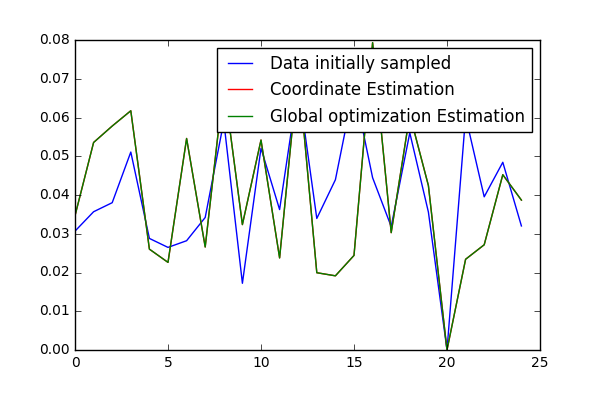
\includegraphics[width=\textwidth,height=\textheight,keepaspectratio]{LambdaEstimationFixedPrior}
		\caption{Lambda Estimation Fixed Prior}
		\label{label-image9}
	\end{figure}
	
	\begin{figure}
		\centering
		%		\textbf{Your title}\par\medskip
		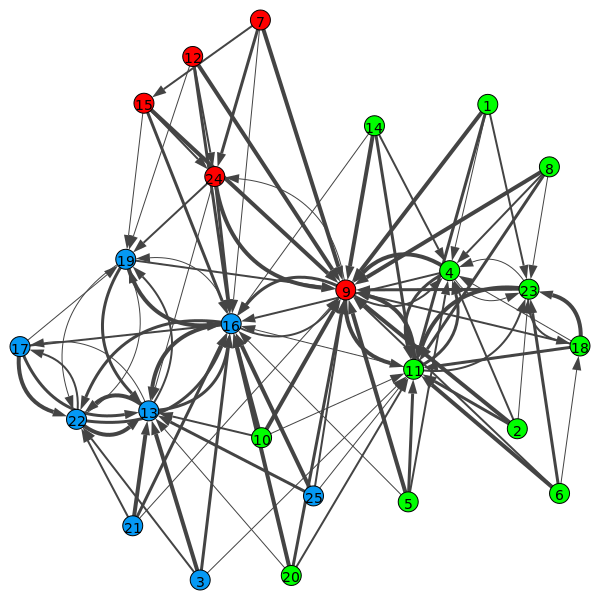
\includegraphics[width=\textwidth,height=\textheight,keepaspectratio]{OriginalPlotFixedPrior}
		\caption{Original Graph}
		\label{label-image10}
	\end{figure}
	
	\begin{figure}
		\centering
		%		\textbf{Your title}\par\medskip
		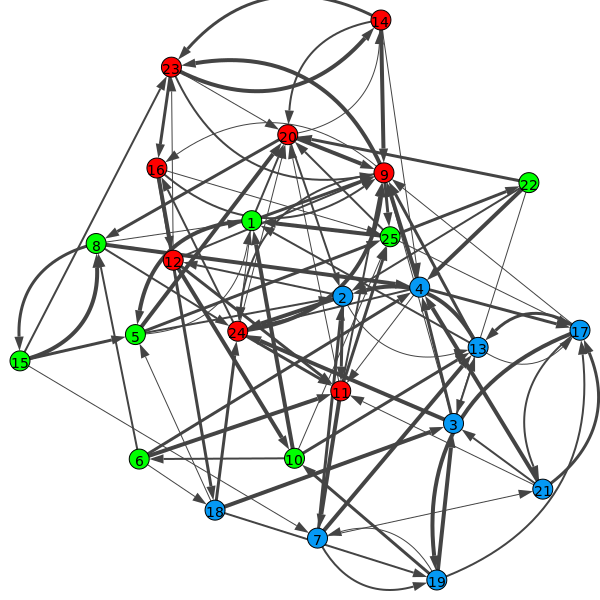
\includegraphics[width=\textwidth,height=\textheight,keepaspectratio]{OptimizationPlotFixedPrior}
		\caption{Inferred Graph}
		\label{label-image11}
	\end{figure}
	
	Now we made a simulation of 10 networks and measured the mean Absolute Error and Ranking Gap.
	
	\begin{figure}
		\centering
		%		\textbf{Your title}\par\medskip
		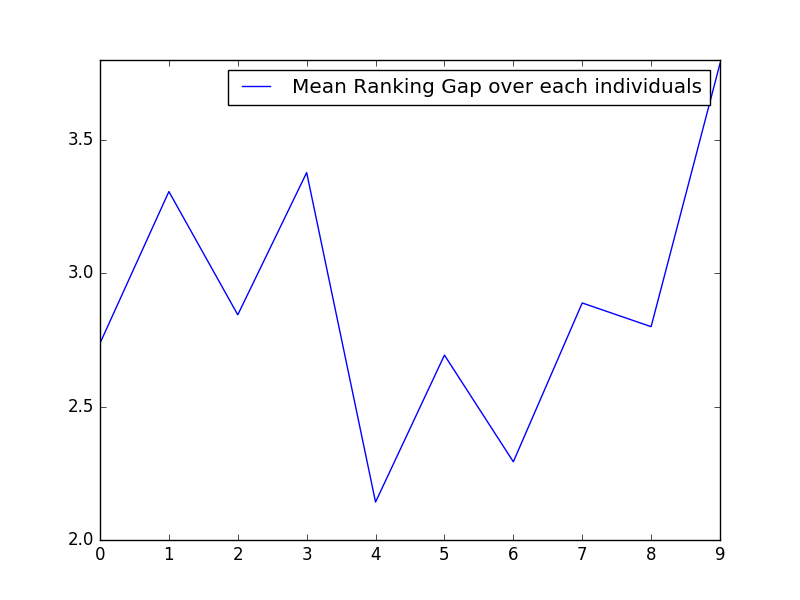
\includegraphics[width=\textwidth,height=\textheight,keepaspectratio]{SimulationGap}
		\caption{Inferred Graph}
		\label{label-image12}
	\end{figure}
	
	We have a mean ranking gap of $2.8871111111111114$ compared to a mean of 5. A a mean AE of $0.022484955968703896$
	
	
	We run for 100 networks with the same parameters.
	We have mean ranking gap of 2.9304888888888896 and mean AE of 0.02122157183931606
	
	\begin{figure}
		\centering
		%		\textbf{Your title}\par\medskip
		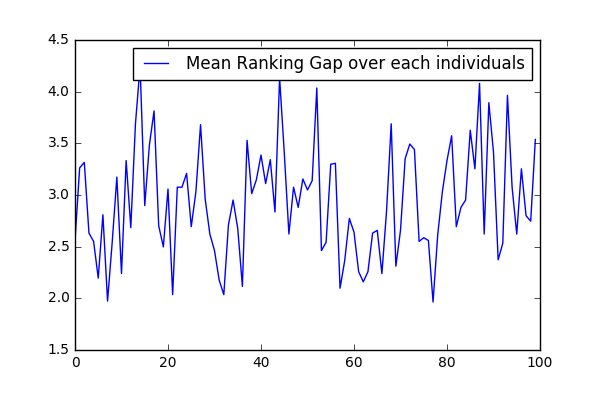
\includegraphics[width=\textwidth,height=\textheight,keepaspectratio]{SimulationGap100}
		\caption{Ranking Gap Community Representation}
		\label{label-image13}
	\end{figure}
	
	
	\section{Model With Degree Correction}
	
	We draw a simulation of 100 networks with $n = 100$, $ p = 3$, $k = 4$, $a = 2$, $b = 2$, optimized it. We obtain the graph with ranking gap of 2.942666666666666 for a mean of 5 and AE of 0.03798207013695899
	
	\begin{figure}
		\centering
		%		\textbf{Your title}\par\medskip
		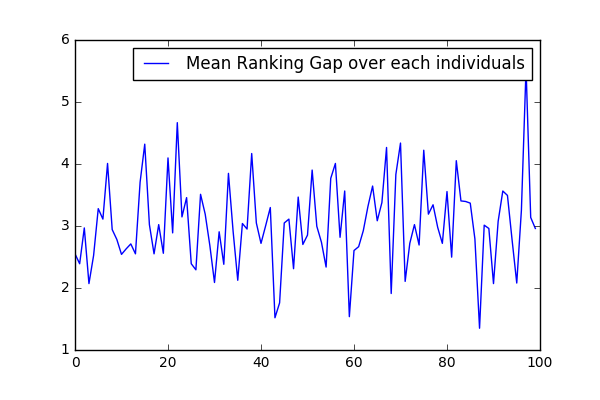
\includegraphics[width=\textwidth,height=\textheight,keepaspectratio]{SimulationGapDegreeCorr}
		\caption{Ranking Gap Degree Correction}
		\label{label-image14}
	\end{figure}
	
	
	\section{Model With Covariates}
	
	We simulated 100 networks of 100 individuals with the rank model:
	
	$y_{i,j} = \beta_{0} + a_{i} + b_{j} + \epsilon_{i,j}$
	
	
	\(
	\begin{pmatrix}
	a_{i} \\
	b_{i}
	\end{pmatrix}
	\), i = 1,...,n $\sim $ i.i.d normal(0,$\Sigma_{ab}$)
	
	\(
	\begin{pmatrix}
	\epsilon_{i,j} \\
	\epsilon_{j,i}
	\end{pmatrix}
	\), i = 1,...,n $\sim $ i.i.d normal(0,$\sigma^{2}$ $\begin{pmatrix} 1 & \rho \\ \rho & 1 \end{pmatrix}$)
	
	
	
	
	\chapter{Simulations on the Sampson’s monk dataset}
	In this part we use the The data set collected by Sampson (1968) this is a classic data set in social network analysis. The data set summarizes relationships, observed at three distinct time points, among 18 monks who were about to enter a monastery when a conflict erupted. We use here the directed network where $y_{i,j} = 1$ denotes that monk i ranked monk j among his top three preferred individuals and $y_{i,j} = 0$ otherwise. The directed network is shown in Figure \ref{label-image4} , where circles represent monks and directed edges are oriented from i to j whenever $y_{i,j} = 1$. The monks are divided by Sampson into three groups: Loyal Opposition, Turks, and Outcasts.
	
	We applied the same method as for the simulated data and obtained the following community. We can observe that our model identifies exactly the same clustering of communities as the ones observed by Sampson. Namely the Loyal Opposition (Red community), Turks (Green Community), and Outcasts (Blue Community). In this graph the individuals are labeled according to their number provided with their names in the data set package and not according to their rank in the data-frame.
	
	
	\begin{figure}
		\centering
		%		\textbf{Your title}\par\medskip
		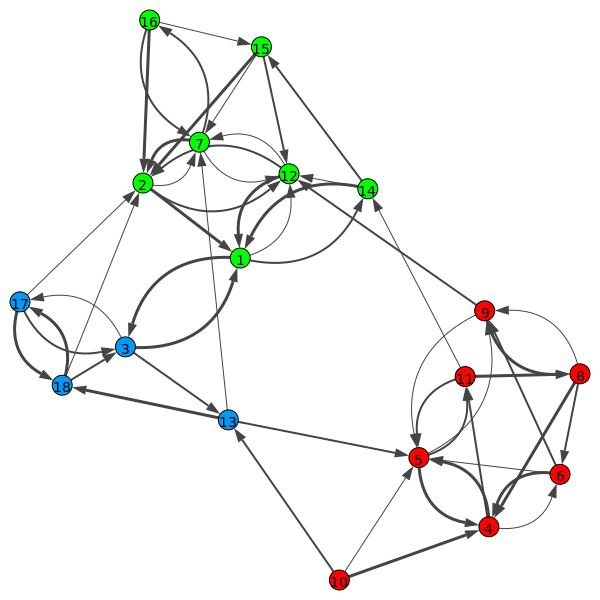
\includegraphics[width=\textwidth,height=\textheight,keepaspectratio]{OptimizationPlotSam}
		\caption{Inferred community for the Sampson DataSet}
		\label{label-image4}
	\end{figure}
	
	
	
\end{document}